\section*{}
\begin{frame}{}
\begin{beamercolorbox}[colsep=1.5pt,rounded=true,shadow=true]{block body example}
    \huge{Chapter 6: Exploiting Channel Correlation against Distance Fraud}
\end{beamercolorbox}
\textbf{Publications:}\\
\begin{small}
    C. Paschou, O. Johnson, A. Doufexi, Z. Zhu, and W.H. Chin. ``Increasing the secrecy gap in quasi-static Rayleigh channels with secret splitting.'' In 2020 IEEE Globecom Workshops (GC Wkshps, pp. 1-7. IEEE, 2020.

    C. Paschou, O. Johnson, Z. Zhu, and A. Doufexi. ``A Lightweight Protocol for Validating Proximity in UHF RFID Systems.'' In 2021 IEEE 94th Vehicular Technology Conference (VTC2021-Fall), pp. 1-7. IEEE, 2021.

    C.Paschou, Z. Zhu, M. Sandell.
    ``Preventing replay/relay attacks in keyless entry systems.'' Patent 54322US, Oblon, McClelland, Maier \& Neustadt, {L.L.P.}, 2022.
    
    \end{small}

\end{frame}


\section{Exploiting channel correlation against distance fraud}

\begin{frame}{Motivation}
\framesubtitle{Authentication in short-range systems}

\begin{figure}
    \vspace{-1cm}
    \hspace*{-1.2cm}
    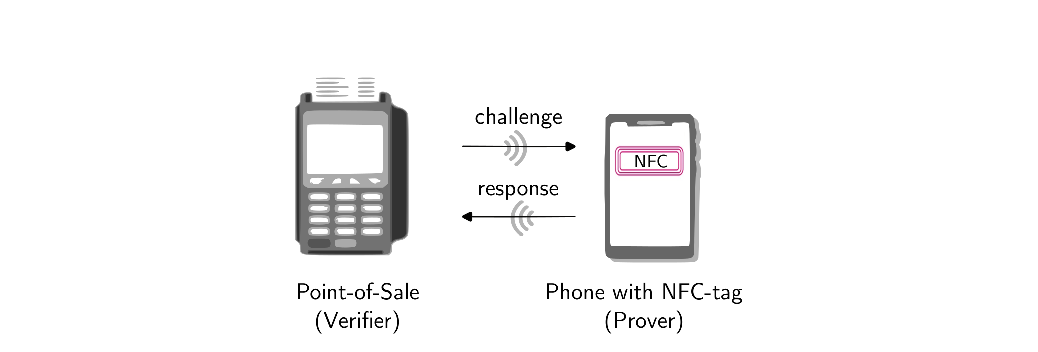
\includegraphics[scale=0.8]{slides/figures/NFC.eps}
    \caption{Verifier-prover example in NFC.}
    \label{fig:NFC}
\end{figure}
\vspace{-1cm}
\begin{beamercolorbox}[colsep=1.5pt,rounded=true,shadow=true]{block body alerted}{Current \textbf{short-range systems} are vulnerable to \textbf{distance fraud}.}
\end{beamercolorbox}
    
\end{frame}

\begin{frame}{Motivation}
\framesubtitle{Mafia-Fraud}
    \begin{figure}
    \hspace*{-2cm}
        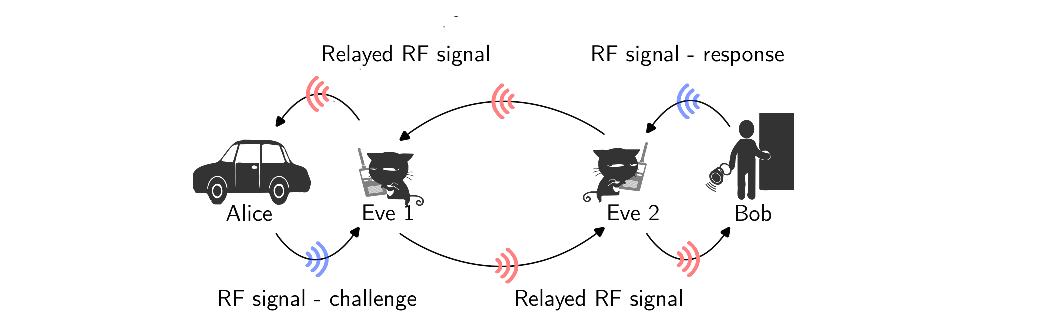
\includegraphics[scale = 0.9]{slides/figures/mafia_fraud.eps}
        \caption{A Mafia Fraud attack with two adversary nodes.}
        \label{fig:enter-label}
    \end{figure}
\end{frame}

\begin{frame}{Terrorist Fraud}
    \begin{figure}
        \centering
        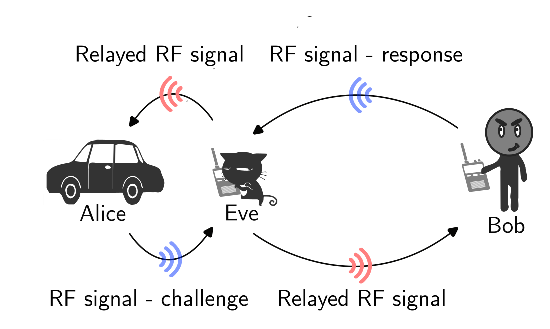
\includegraphics[scale = 0.9]{slides/figures/terrorist_fraud.eps}
        \caption{In a Terrorist Fraud attack, remote Bob cooperates with a local adversary node.}
        \label{fig:enter-label}
    \end{figure}
\end{frame}



\begin{frame}{Motivation}

\framesubtitle{Current Solutions and Limitations}
    \begin{itemize}
        \item Physical Layer Identification - promising solution against most distance fraud;
        \item Time-of-flight distance bounding - best solution but requires specialised hardware;
        \item Ambient Conditions - at least 5 sensor devices are needed;
        \item RSS and phase-based ranging - easy to implement but extremely vulnerable. AVOID.
    \end{itemize}
\vspace{2pt}
\begin{beamercolorbox}[colsep=1.5pt,rounded=true,shadow=true]{block body alerted}
A reliable method for narrowband and low-cost devices is missing.
\end{beamercolorbox}
\end{frame}

\begin{frame}{Motivation}
\framesubtitle{Our solution}

\begin{itemize}
\item Exploit the inherited properties of the RF channel: spatial/temporal correlation.
\item Two variants:
\begin{itemize}
    \item CHannel Randomness Yields Secure Proximity (\textbf{CHRYSP})
    \item against Solo-Distance RFID (\textbf{SD-RFID})
    \end{itemize}

\end{itemize}

    
\end{frame}


\begin{frame}{Motivation}
\framesubtitle{Our Solution vs Current Solution}
\begin{table}[ht!]
    \centering
    \begin{tabular}{|c|c|c|c|c|}
    \hline
     & Replay& Solo Dist.& Mafia& Terrorist\\
      & attack& Fraud& Fraud& Fraud\\
     %\hline
     %Crypt. methods & \checkmark& X& X&X   \\
     \hline
     RF fingerprints & \checkmark& X& \checkmark& \checkmark\\
     \hline
     Ambient Conditions & \checkmark& \checkmark&\checkmark & X\\
        \hline
     Time-of-flight& X& \checkmark &\checkmark & {\small{depends on}}\\
     dist. bound.&&&&\small{protocol}\\
     \hline
     CHRYSP & \checkmark & \checkmark &\checkmark & X\\
     \hline
     SDF-RFID & \checkmark & \checkmark &X& X\\
     \hline
    \end{tabular}
        \caption{Possibility for protection against authentication attacks in short-range communication systems}
    \label{tab:attacks}
\end{table}

\end{frame}


\begin{frame}{CHRYSP}
\framesubtitle{Channel Model}
\begin{figure}
    \centering    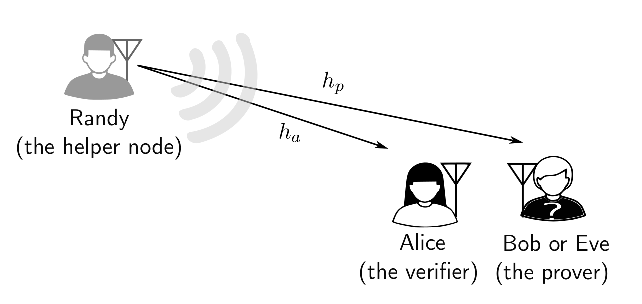
\includegraphics{figures/against_distance_fraud/RandyAliceChannelmodel.eps}
    
    \caption{Randy, Alice and Bob/Eve play the role of the helper node, the verifier, and the prover, respectively.}
\end{figure}
\end{frame}
%%%%%
\begin{frame}
\centering
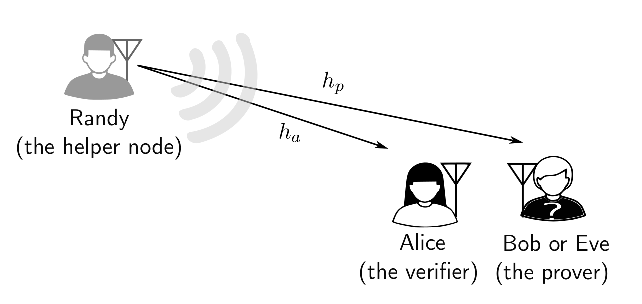
\includegraphics[width=0.6\linewidth]{figures/against_distance_fraud/RandyAliceChannelmodel.eps}

\begin{enumerate}
\item<1-> \textit{Channel measurements.}
Randy transmits known symbols. 
Alice \& prover record $N$ independent realisations of $h_a$ and $h_p$. Alice's and prover's channel sequences: $\{h_a[i]\}$, $\{h_p[i]\}$.

\item<2-> \textit{Signature.} The prover signs the channel sequence. Both channel sequence and signature are sent to Alice.


\item<3-> \textit{Legitimacy test.} Alice checks the validity of the signature.

\item<4-> \textit{Proximity test.} Alice estimates the channel correlation  $R(h_a, h_p)$. For a given threshold $\tau$:
\begin{align}
    &\text{If } |\hat{R}|\geq \tau, \text{ accept the prover}; \nonumber\\
    &\text{Otherwise}, \text{ reject the prover}.\nonumber
\end{align}
\end{enumerate}
\end{frame}

%%%%%%%%%%%%%%%%%%%%%%%%%%%%%%%%%%

\begin{frame}{SD-RFID}
\framesubtitle{Channel model}
\begin{figure}
    \vspace{-1cm}    
    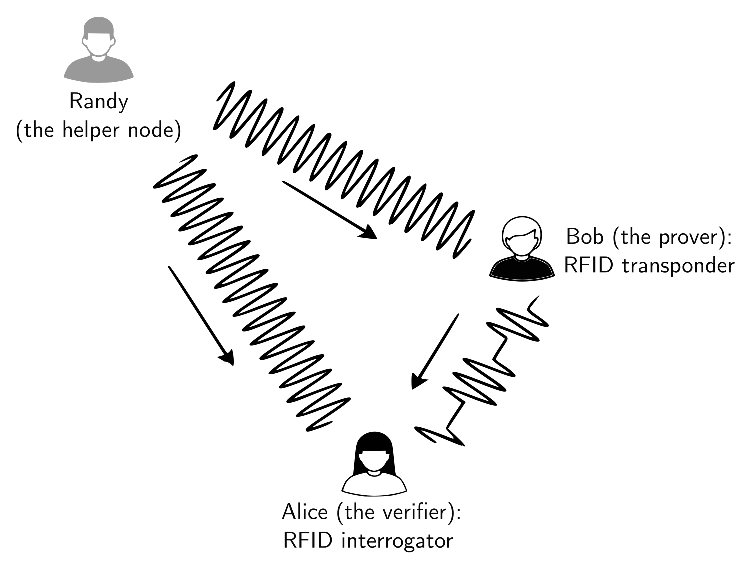
\includegraphics[scale = 0.6]{figures/against_distance_fraud/superposition.eps}
    \caption{The interrogator receives the superposition of two transmitting signals. At times when the transponder does not reflect the interrogator evaluates the channel $h_a$, whereas $h_b$ is measured during reflection.}
    \label{fig:enter-label}
\end{figure}
    
\end{frame}

\begin{frame}{Concluding Remarks}
\begin{itemize}
    \item The spatial channel correlation properties can be exploited to prove proximity.

    \item Under perfect channel estimation, the suggested method is a promising solution against relay attacks in non-static environments.

    \item A channel rich in entropy allows the required minimum channel correlation to be a small value, thereby enabling authentication over longer distances.

\end{itemize}
\end{frame}

\begin{frame}{Methodology}
\begin{enumerate}
    \item \textit{Data transmission.} Bob transmits typical data to Alice by using backscattering modulation on Randy's signal; 
    \item \textit{Channel measurements.} By applying signal processing techniques, Alice estimates both her own channel and Bob's channel. 
    \item \textit{Proximity Test.} Alice estimates the spatial channel correlation and approves or rejects the prover accordingly.  
\end{enumerate}
    
\end{frame}

\begin{frame}{Differences between SD-RFID \& CHRYSP}
\centering
\begin{tabular}{|p{2.5cm}|p{4cm}|p{3.5cm}|}
\hline
& \textbf{SD-RFID} & \textbf{CHRYSP} \\
\hline

\textbf{at the prover} & performs backscattering & RF antenna \\
 & seamless application & additional actions\\
\hline
\textbf{resilience} & SD-fraud & SD-fraud \\
 against& replay attack & replay attack \\
 \textbf{attacks}&               & Mafia Fraud \\
\hline

\end{tabular}
    
\end{frame}

\begin{frame}{Numerical Results}
\begin{figure}
    \centering
    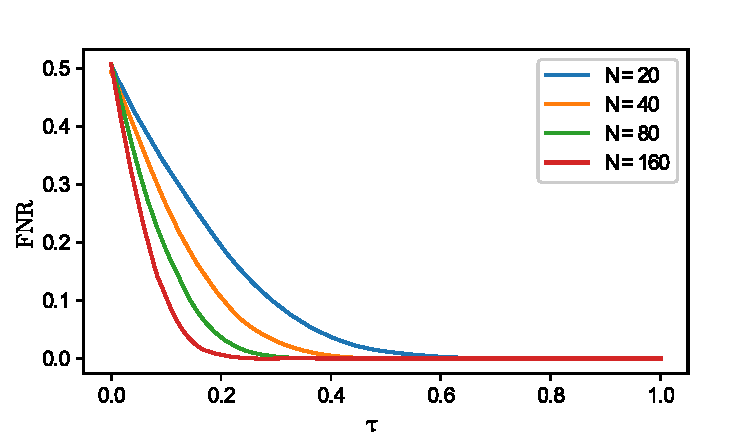
\includegraphics[scale = 0.8]{figures/against_distance_fraud/FNR_protect.eps}
    
    \caption{False-negative rate against the decision threshold}
\end{figure}
\end{frame}


\begin{frame}{Numerical Results}
\begin{figure}
    \centering
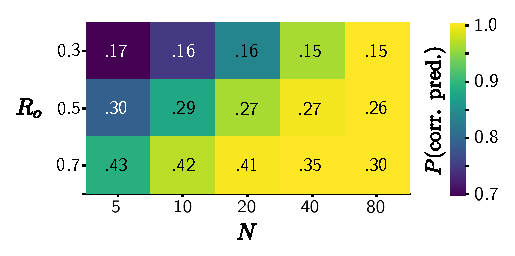
\includegraphics{figures/against_distance_fraud/colourmap_inkscape.eps}
\caption{Optimal thresholds for increasing the probability of correct predictions.}
\end{figure}
        
\end{frame}

\begin{frame}{Numerical Results - Insights}
\begin{itemize}

    \item Under perfect channel estimation and non-static environments, CHRYSP and SDF-RFID can protect against authentication attacks in short-range systems;
    \item A channel rich in entropy allows the required minimum channel correlation to be a small value, thereby enabling authentication over longer distances;
    

\end{itemize}

\end{frame}

\begin{frame}{Concluding Remarks}
\begin{itemize}

    \item Motivated by real-life authentication attacks in short-range systems, a novel concept has been introduced:\\
    Exploit channel correlation
    \item No specialised hardware, multiple sensors, or UWB systems are required except for the existence of a helper node and a non-static environment;
    \item Proposed methods are a good fit for resource-constrained short-range systems.
    

\end{itemize}

\end{frame}


